% Compile with: latexmk -pdfxe -outdir=build
\documentclass[12pt,oneside]{LuThesis}
\usepackage[dvipsnames]{xcolor}
\definecolor{bostonuniversityred}{rgb}{0.8, 0.0, 0.0}
\definecolor{awesome}{rgb}{1.0, 0.13, 0.32}
\definecolor{cadmiumgreen}{rgb}{0.0, 0.42, 0.24}
\usepackage{listings}
\lstset{language=R,%
    %basicstyle=\color{red},
    basicstyle=\ttfamily,%
    breaklines=true,%
    morekeywords={matlab2tikz},
    keywordstyle=\color{blue},%
    morekeywords=[2]{1}, keywordstyle=[2]{\color{black}},
    showstringspaces=false,%without this there will be a symbol in the places where there is a space
    numbers=left,%
    numberstyle={\tiny \color{black}},% size of the numbers
    numbersep=9pt, % this defines how far the numbers are from the text
    emph=[1]{for,in,end,break},emphstyle=[1]\color{bostonuniversityred}, %some words to emphasise
    %emph=[2]{word1,word2}, emphstyle=[2]{style}, 
    emph=[1]{data.frame},emphstyle=[1]\color{awesome}, %some words to emphasise   
}

\title{Saules paneļu efektivitāte Latvijas klimatā}
\author{Viktorija Leimane}

%%% LuThesis deklerācijas
\def\studaplnum{vl16047}
\def\darbvad{Dr. Phys. Andris Jakovičs}
\def\dokfak{\textbf{Fizikas, matemātikas un optometrijas fakultāte}}
\def\recenzents{Dr. Phys.Aivars Vembris}
\def\doktitle{\textbf{Saules paneļu efektivitāte Latvijas klimatā}}
\def\dokfak{\textbf{Fizikas, matemātikas un optometrijas fakultāte}}
\def\dokdate{} % Darba vadītāja parakstīšanas datums
\def\dokdateiesn{} % Darba iesniegšanas datums

%%% Valodas un fonti
\setdefaultlanguage{latvian}
\setotherlanguage{english}
\setmainfont[BoldFont=FreeSerifBold.ttf,ItalicFont=FreeSerifItalic.ttf,BoldItalicFont=FreeSerifBoldItalic.ttf]{FreeSerif.ttf}

\usepackage{graphicx}

%%% Misc
% \usepackage{hyperref}
\usepackage[hidelinks]{hyperref}
\addbibresource{bachelor.bib} % biblatex bibliotēkas fails: bachelor.bib
\usepackage[section]{placeins}
\usepackage[toc,page]{appendix}

%%% Dokumenta struktūra
\begin{document}

\maketitle

% * Anotācija
\chapter*{Anotācija}
\setcounter{page}{1}
\begin{abstract}
Darba mērķis ir noteikt efektīvāko saules paneļu izvietojuma veidu Latvijai tipiskos meteoroloģiskajos apstākļos. 
Balstoties uz divu veidu saules paneļiem, kas novietoti piecās dažādās telpiskajās orientācijās Latvijas Universitātes Botāniskā dārza teritorijā, tiks noteikta solāro paneļu efektivitātes atkarība no mainīgiem parametriem:
1) meteoroloģiskie apstākļi
2) telpiskā orientācija
3) gada mēnesis
4) solāro paneļu tips. \\
Iegūtie monitoringa rezultāti tiks analizēti kontekstā ar šo paneļu efektivitātes fizikālo novērtējumu.\\

\keywords{Saules enerģijas paneļi, atjaunojamo energoresursu enerģija, vides monitorings}
\end{abstract}

\chapter*{Abstract}
\begin{english}
\begin{abstract}
The aim of this thesis is to determine the most efficient way of solar panel arrangement for the climatic conditions of Latvia.
Based on two types of solar panels placed in five different spatial orientations in the University of Latvia Botanical Garden area, the dependency of the efficiency of solar panels on following variable parameters is established:
\begin{enumerate}
\item type of solar panels
\item spatial orientation
\item month of year
\item meteorological conditions.
\end{enumerate}

The results of the monitoring are analysed in the context of solar irradiance intensity, the physical assessment of the partial(?) efficiency of the panels and the results of other measurements.

\keywords{Solar panels, renewable energy}
\end{abstract}
\end{english}

%* Saturs
\tableofcontents

%* Apzīmējumu saraksts
\chapter*{Apzīmējumu saraksts}
\addcontentsline{toc}{chapter}{Apzīmējumu saraksts}
\noindent 
\textbf{Klimats}\\
TSI - Kopējais saules apstarojums, $\textrm{Wm}^{-2}$\\
SSI - Saules spektrālais apstarojums, $\textrm{Wm}^{-2}\textrm{nm}^{-1}$\\
% $G_{sc}$ - Solārā konstante, $\textrm{Wm}^{-2}$\\
%Photovoltaic power potential
TIM - Kopējā apstarojuma novērotājs\\
GHI – Globālais horizontālais apstarojums,  $\textrm{kWh/m}^2$\\ %Global horizontal irradiation
DHI – Difūzais horizontālais apstarojums,  $\textrm{kWh/m}^2$\\ 
DNI – Tiešais normālais apstarojums, $\textrm{kWh/m}^2$\\ %Direct normal irradiation
CMF - Mākoņu modifikācijas reizinātājs\\
AU - astronomiskā vienība\\  %astronomical unit
\textbf{Saules kustības leņķi}\\
$\theta$ - staru krišanas leņķis uz saules paneli\\
$\delta$ - Saules deklinācija -- leņķis starp virzieniem uz Sauli un debess ekvatoru solārajā pusdienlaikā.\\
 $\phi$  - ģeogrāfiskais platums; pozitīvs Z virzienā.\\
$\beta$  - paneļa slīpums -- leņķis starp Saules paneļa virsmu un horizontāli.\\
$\gamma$ - paneļa azimuts -- leņķis starp virsmas normāles projekciju uz horizontālo  plakni un D virzienu.\\
$\omega$ - solārais stundu leņķis -- leņķis starp Saules stara virziena projekciju uz horizontālo plakni un D virzienu; negatīvs no rīta.\\
\textbf{Saules paneļi}\\
PV - fotoelektriskais elements\\ %fotogalvanisks?
Si - silīcijs\\
P - jauda, 	W\\
Pmax - maksimālā jauda, W\\
PVOUT – Saules fotoelementa potenciālā jauda, $\textrm{kWh/kWp}$\\ 
%Photovoltaic power potential
E$_{norm}$, $\textrm{kWh/m}^2$ - enerģija normēta uz saules paneļa laukuma vienību.\\
\textbf{Debespuses}\\
A - austrumi\\
R - rietumi\\
D - dienvidi\\

%* Ievads
\chapter*{Ievads}
\addcontentsline{toc}{chapter}{Ievads}
Apvienoto Nāciju Organizācijas Klimata konferencē Parīzē 2015. gada decembrī daudzas pasaules valstis vienojās ierobežot globālo sasilšanu zem 2\textdegree C salīdzinājumā ar pirmsindustriālo laikmetu.
%, tāpēc ES ir apņēmusies līdz 2030. gadam samazināt siltumnīcefekta gāzu emisijas vismaz par 40\% salīdzinājumā ar 1990. gada līmeni.
Tāpēc Eiropas Savienībā noteikts dalībvalstīm saistošs mērķrādītājs  –  vismaz 32\%  atjaunojamās enerģijas īpatsvars līdz 2030. gadam \cite{ES}.

Ne mazāk būtiska ir atjaunojamo energoresursu loma energoapgādes neatkarības un drošības veicināšanā, tehnoloģiju attīstībā un inovācijās, vienlaikus sniedzot labumu videi un sabiedrībai, kā arī nodrošinot svarīgus priekšnosacījums nodarbinātībai, reģionālajai attīstībai un elektrības nodrošināšanai grūti pieejamās vietās \cite{ES}.

Dažādu atjaunojamo enerģijas resursu - saules, vēja, ģeotermālo un ūdens - starpā Saules enerģija ir viens no kandidātiem klimata pārmaiņu un to seku mazināšanai un efektīvas energoapgādes nodrošināšanai. Pēdējā desmitgadē veiktās investīcijas Saules enerģijas izmantošanā manifestējās inovācijās saules paneļu ražošanā, un gala rezultātā tie ir kļuvuši efektīvāki un finansiāli pieejamāki patērētājiem, piemēram, silīcija saules paneļu cena sastāda $\leq$ 30\% no kopējām saules paneļu sistēmas uzstādīšanas izmaksām un to saražotā enerģija atkarībā no atrašanās vietas un paneļa veida atmaksājas pēc $\geq$ 3 gadu perioda \cite{researchOpp}. Tomēr bez klimata to efektivitāti ietekmē arī daudzi citi faktori, kas tiek analizēti šajā darbā, piemēram, saules paneļu tips un telpiskā orientācija.

Šī pētījuma \textbf{mērķis} ir analizēt un praktiski pārbaudīt divu tipu (JA un LG) saules paneļu efektivitāti atšķirīgos telpiskās orientācijās risinājumos -- pētītas trīs dažādu virzienu (dienvidu (D), rietumu (R), austrumu (A)) un trīs leņķu pret horizontu (13\textdegree, 40\textdegree, 90\textdegree) paneļu grupas -- un tiek salīdzināta to piemērotība Latvijas klimatiskajiem apstākļiem.

% \subsection{Darba uzdevumi}
\textbf{Darba uzdevumi}
\begin{itemize}
\item Ievākt, atlasīt un analizēt saules paneļu jaudas (P) datus.
\item Izveidot iespējami automatizētu datu apstrādes sistēmu R valodā ilgtermiņa montioringa vajadzībām.
\item Salīdzināt paneļu efektivitāti gada laikā mēnešu intervālos atbilstoši tipa un telpiskās orientācijas apakšgrupām.
% \item Balstoties uz ilgtermiņa saules izstarojuma monitoringu, novērtēt saules paneļu saražoto enerģiju no fizikālajiem apsvērumiem.
\item Novērtēt datu kvalitāti no fizikālo apsvērumu un saules apstarojuma mērījumu viedokļa.
\end{itemize}

% \subsection{Darba aktualitāte}
\textbf{Darba aktualitāte}

Darba nozīme atklājas detalizētas paneļu efektivitātes analīzes nepieciešamībā tieši Latvijas klimatiskajiem apstākļiem. Latvijā veikto pētījumu daudzums un kvalitāte pagaidām neļauj iegūt pilnīgu priekšstatu par Saules paneļu lietošanas iespējām un prognozēt dažādu paneļu tipu efektivitāti reālā Latvijas klimatā. Tāpēc šī darba novitāte ietverta programmatūras izveidē, kas ļauj attēlot un apstrādāt Saules paneļu monitoringa datus, kas dos iespēju veikt turpmākus dziļākus pētījumus par dažādiem saules paneļu spēkstaciju pielietojuma aspektiem Latvijā.\\
% \subsection{Darba struktūra}

\textbf{Darba struktūra}

Darba pirmo daļu veido literatūrā pieejamo Saules apstarojuma novērtējumu raksturojums un apskats par Saules redzamo pārvietošanās pie debess sfēras diennakts laikā 60 dienu intervālos. Otrajā daļā aplūkota saules paneļu uzbūve un to darbības princips. Trešajā daļā tiek apskatīta saules paneļu sistēmas elektriskā shēma un raksturoti LU Botāniskā dārza spēkstacijas instalācijas parametri.
Ceturtajā daļā ir aprakstīti iegūtie rezultāti, tie ir salīdzināti savā starpā, ar citas saules paneļu spēkstacijas mērījumu rezultātiem, ar eksperimentālā poligona meteostacijas datiem par solāro apstarojumu šajā laika periodā, kā arī aplūkoti no teorētiskās pusvadītāju fizikas aspektiem.\\

\textbf{Autores ieguldījums darbā}
% \subsection{Autores ieguldījums darbā}
% the \\ insures the section title is centered below the phrase: Appendix B

Saules paneļu uzstādīšanu veica SIA EG Inženieri Valda Gailīša vadībā.
Par datu ievākšanu no saules paneļu sistēmas datu uzkrājējiem jāpateicas Victron Energy B.V. izstrādātājai VRM sistēmai.

Mans ieguldījums ir koda arhitektūras plānošana, rakstīšana un uzturēšana līdz šim brīdim. Esmu vienīgais koda bāzes izstrādātājs. Darbā kopā veikti 318 iesūtījumi (\textit{commits}) trīs zaros (105, 123 un 90 iesūtījumi attiecīgi), kas rezultējās 3140 koda rindās. 

Darba gaitā veicu datu lejupielādi, datu informācijas aptveršanu, kā arī datu programmatisku atlasīšanu, apstrādi, apkopošanu, transformēšanu vizualizācijas vajadzību pielāgošanai un datu vizualizāciju. 

% \begin{figure}[h]
% 	\centering
% 	\includegraphics[width=0.6\linewidth]{figures/misc/contributions.png}
% 	\caption{Darba autores ieguldījums master zarā.}
% 	\label{fig:retribution}
% \end{figure}
% % TEORIJAS KOPSAVILKUMS
Vispirms tiek aplūkota Saules emitētā starojuma daba un ģeometriskie apsvērumi - virziens, no kura staru kūlis sasniedz virsmu, leņķis uz virsmas un laika gaitā saņemtais starojuma daudzums. Tiek apskatīta atmosfēras un mākoņu ietekme uz virsmas saņemto saules starojumu, un tās praktiskā nozīme, apstrādājot pieejamos Saules starojuma datus, lai aprakstītu radiācijas gadījumus uz virsmas dažādās orientācijās.

% atjaunojamā enerģija
% kāpēc ir svarīgi
% 	politika (direktīva)
% 	klimata pārmaiņas
% atjaunojamās enerģijas veidi (vējš, saule, utml)
% mērķis ir salīdzināt solāro paneļu saražoto enerģiju atkarībā no modeļa, telpiskās orientācijas, leņķa un kā mainās pa gadalaikiem tieši latvijā
% citos klimatiskajos apstākļos līdzīgas analīzes ir veiktas ko var iegūt dažādās klimatiskajās zonās
% pierakstīt par pv paneļu darbību un efektivitāti
% aprakstīt ko tu darīji, lai pēc iespējas automatizētu datu apstrādes sistēmu
% kādus datus uzkrāj kādā attēlojumā
% datu menedžmentu aprakstīt
% paskatīties kā nosaka solāro paneļu efektivitātes standartu
% sarēķināt attiecības starp paneļu saražoto (normēt uz lielāko paneli)
% ielikt grafikus no februāra un aprīļa
% pierakstīt salīdzinājumu
% aprakstīt gļukus, kur dienā nav nekā saražots bet blakus ir. tā gadās.
% nomaini februāra sol_month grafikos virsrakstu uz februāri
% nomaini $Em^-2$ uz $E_norm$

% * Literatūras apskats
\chapter{Literatūras apskats}
% \section{Definīcijas}
Saules plankums - magnētiskās plūsmas koncentrācija bipolāros klāsteros vai grupās, kas novērojama kā tumšs plankums uz Saules fotosfēras.\\
Saules plankumu cikls - aptuveni 11 gadus ilga kvaziperiodiska variācija saules plankuma skaitlī. Magnētiskā lauka polaritātes modelis mainās ar katru ciklu.\\
Saules plankuma skaitlis - Dienas saules plankuma aktivitātes indekss (R), definēts kā R = k(10g + s), kur
s - individuālo plankumu skaits;
g - saules plankumu grupu skaits;
k - observatorijas faktors.
total solar irradiance (TSI) - Solar energy per unit time over a unit area perpendicular to the Sun’s rays at the top of Earth’s atmosphere.
% \\http://lasp.colorado.edu/home/sorce/reference/glossary/
\input{tex/literatura}
\section{Saules apstarojums}

Lielākā daļa Saules izstarotās enerģijas tiek saražota kodolreakcijās fotosfērā. 
Kopējais saules apstarojums (\textit{Total Solar Irradiance}, TSI) raksturo Saules starojuma absolūto intensitāti -- enerģiju uz virsmas perpendikulāri starojuma izplatīšanas virzienam 1 AU attālumā no Saules, integrētu visā saules enerģijas diskā un visā saules enerģijas spektrā. TSI vērtībai novērojama aptuveni 11 gadus ilga periodiska variācija, kas korelē ar saules plankumu skaitli (\ref{fig:TSI_misijas}. att.). Par Saules plankumu sauc magnētiskās plūsmas koncentrāciju bipolāros klāsteros vai grupās izraisītos tumšos plankums uz Saules fotosfēras, savukārt Saules plankumu skaitlis ir atkarīgs no individuālu Saules plankumu $s$ un to grupu $g$ skaita, kā arī observatorijas atrašanās vietas faktora $k$
pēc~\ref{eq:aktivitatesIndex} formulas~\cite{ThermalProcesses}.

\begin{equation}
\label{eq:aktivitatesIndex}
R = k(10 \cdot g + s)
\end{equation}

TSI norāda uz solārās radiācijas izmaiņām, kas ietekmē Zemes atmosfēras augšējos slāņos saņemto solārās enerģijas apjomu. Papildus ir noderīgi zināt Saules emitētā starojuma spektrālo sadalījumu (\textit{Spectral Solar Irradiance}, SSI) -- \ref{fig:SSI}. att. redzams, ka aptuveni puse starojuma tiek saņemta salīdzinoši maza viļņu garumu - 380 -- 780 nm diapazonā~\cite{ThermalProcesses}.
 % kas padara iespējumu no tā iegūt enerģiju ar saules paneļu paņēmienu pēc formulām \ref{eq:proof}. 
% kādēļ tieši šis diapazons?
% atradu cik šī diapazona laukums ir procenti no visa laukuma un negribēju rēķināt citu
% mazs viļņu garums, tātad ar lielu frekvenci, tātad daudz enerģijas
% \begin{equation}
% \label{eq:proof}
% \nu \uparrow = \frac{c}{\lambda \downarrow} \qquad E \uparrow = h \nu \uparrow 
% \end{equation}

TSI novērojumi no kosmosa tiek veikti kopš 1978. gada un instrumentu specifikas dēļ iegūtas dažādas absolūtās vērtības (skat. att. \ref{fig:TSI_misijas}.), tāpēc šī fizikālā lieluma tikai daļēji pārkājušos novērojumu laikrindu apvienošana kompozītā ir gan zinātnisks, gan statistisks izaicinājums un neviens kompozīts (piemēram, PMOD, ACRIM, IRBM) līdz šim nav kļuvis par absolūtu standartu solārā apstarojuma pētnieku kopienā~\cite{Frohlich2012}.

\begin{figure}[h]
    \centering
    \includegraphics[width=\linewidth]{figures/misc/TSI_misijas.png}
    \caption{Salīdzinājums dienā vidējotiem saules kopējā apstarojuma datiem no dažādām kosmiskajām misijām un Saules plankuma skaitlis, lai ilustrētu solārās aktivitātes variabilitāti trīs ciklos \cite{Frohlich2012}.}
    \label{fig:TSI_misijas}
\end{figure}

Par labāko Saules apstarojuma mērījumu reprezentāciju tiek uzskatīti Saules Radiācijas un Klimata Eksperimenta (\textit{Solar Radiation and Climate Experiment}, SORCE) misijas kopējā apstarojuma novērošanas instrumenta (\textit{Total Irradiance Monitor}, TIM)  dati mēraparāta uzbūves -- atšķirībā no citiem radiometriem TIM precizitātes apertūra atrodas tuvu dobumam un redzeslauku bloķējošā apertūra ir pie instrumenta ieejas -- un augstās precizitātes -- nenoteiktība tiek novērtēta esam mazāk nekā $0.014$ $\textrm{W  m}^{-2}\textrm{yr}^{-1}$ un precizitāte ar $0.48$ $\textrm{W  m}^{-2}$ \cite{TSIdata} -- dēļ, tāpēc šajā darbā grafiki balstās uz šiem mērījumiem, pēc kuriem absolūtā kopējā saules apstarojuma vērtība ir $(1360.8 \pm 0.5) \textrm{W m}^{-2}$ ~\cite{Frohlich2012}.

\begin{figure}[h]
    \centering
    \includegraphics[width=\linewidth]{figures/misc/SSI.pdf}
    \caption{SSI 1AU attālumā (24 h vidējā vērtība) \cite{SSIdata}.}
    \label{fig:SSI}
\end{figure}

\begin{figure}[h]
    \centering
    \includegraphics[width=\linewidth]{figures/misc/TSI_8-19.pdf}
    \caption{TSI 24. saules ciklā 1 AU attālumā (24 h vidējā vērtība)\cite{TSIdata}.}
    \label{fig:TSI1}
\end{figure}
% intensity
% spectral distribution
% solar geometry
% saules stāvoklis debesīs
% un virziens, kurā stara starojums krīt uz dažādu virzienu un ēnojuma virsmām

\section{Saules diennakts kustība}\label{section:kustiba}

Šajā nodaļā Saules apstarojums tiek aplūkots no ģeometriskajiem apsvērumiem - virziena, no kura staru kūlis sasniedz virsmu, leņķi uz virsmas un gada gaitā saņemtā starojuma daudzuma.

Ģeometriskās sakarības starp saules paneļa virsmas plakni un ienākošo Saules starojuma kūli jeb Saules pozīcija relatīvi pret šo plakni tiek aprakstīta ar vairākiem leņķiem. Ar $\theta$ apzīmēsim staru krišanas leņķi uz saules paneli, pieņemot saules paneli par nekustīgu plakni. Tad, pie nemainīgas starojuma intensitātes, paneļa saņemtā enerģija būs proporcionāla $\cos{\theta}$ (ja $\theta<90^\circ$) vai būs vienāda ar 0 (ja $\theta \geq 90^\circ$, t.i., Saules stari krīt uz paneļa apakšējo virsmu) pēc formulas \ref{eq:apgaismojums}. Saules diennakts kustība, gadalaiku cikls, kā arī saules paneļa novietojums ir ievēroti $\cos{\theta}$ aprēķina izteiksmē \ref{eq:theta}, kur lietotie leņķi definēti \ref{tab:theta}. tabulā~\cite{ThermalProcesses}.

\begin{equation}
\label{eq:apgaismojums}
E = I \cdot cos(\theta)
\end{equation}
\begin{equation}
\label{eq:theta}
\begin{aligned}
\cos{\theta} = {} & \sin{\delta} \sin{\phi} \cos{\beta} - \sin{\delta} \cos{\phi} \sin{\beta} \cos{\gamma} +                           \\
	& \cos{\delta} \cos{\phi} \cos{\beta} \cos{\omega} + \cos{\delta} \sin{\phi} \sin{\beta} \cos{\gamma} \cos{\omega} + \\
	& \cos{\delta} \sin{\beta} \sin{\gamma} \sin{\omega},
\end{aligned}
\end{equation}

Saules deklināciju solārajā pusdienlaikā var aprēķināt pēc lietderīgas aproksimācijas, kur $n$ apzīmē dienas kārtas numuru gadā. \cite{cooper1969}.
\begin{equation}
\label{eq:delta}
    \delta = 23 \sin \left( 360 \cdot \frac{284+n}{365} \right),
\end{equation}

Ar vienādojumu \ref{eq:theta} un \ref{eq:delta} palīdzību ir iespējams aprēķināt $\cos{\theta}$ laika atkarību, kas ir pirmais tuvinājums Saules apstarojuma izmaiņām dienas laikā.
Parametru vērtības katram no darbā lietotajiem Saules paneļiem ir apkopotas \ref{tab:param}. tabulā.
Lietojot šos parametrus, tika aprēķināta $\cos{\theta}$ atkarība no laika trīs datumiem: 1. janvārim, 1. martam un 30. aprīlim (skat. \ref{fig:cos-theta}. att.). No tā secināms, ka austrumu virzienā uzstādītais panelis saņem vairāk apstarojuma no rīta nekā rietumu virzienā vērstais panelis. Pēc šī aprēķina iespējams prognozēt paneļu saražotās enerģijas izmaiņas gada griezumā, piemēram, no dienvidu paneļiem janvārī efektīvākais ir 90$^\circ$ leņķī vērstais, jo Saule atrodas zemu pie horizonta, bet aprīlī efektīvākais ir 40$^\circ$ leņķī.

\begin{table}[h!]
\caption{Leņķu, kas lietoti \ref{eq:theta} vienādojumā, definīcijas.}
\begin{center}
\begin{tabular}{|c|c|l|}\hline
	         &         Apgabals         & Definīcija\\ \hline
	$\theta$ &  $(0^\circ;180^\circ)$   & staru krišanas leņķis uz Saules paneli\\ \hline
	$\delta$ &  $(-23^\circ;23^\circ)$  & Saules deklinācija\\ \hline
	 $\phi$  &  $(-90^\circ;90^\circ)$  & ģeogrāfiskais platums\\ \hline
	$\beta$  &  $(0^\circ;180^\circ)$   & paneļa slīpums \\ \hline
	$\gamma$ & $(-180^\circ;180^\circ)$ & paneļa azimuts \\ \hline
	$\omega$ & $(-180^\circ;180^\circ)$ & solārais stundu leņķis\\ \hline
\end{tabular}
\end{center}
\label{tab:theta}
\end{table}

\begin{table}[h!]
	\caption{Darbā lietotajiem Saules paneļiem atbilstošās leņķisko parametru vērtības, grādos.}
	\begin{center}
		\begin{tabular}{|r|c|c|c|c|c|}
			\hline
			         & R.13 & A.13 &   D.13   & D.40 & D.90 \\ \hline
			paneļa slīpums $\beta$  & \multicolumn{3}{c|}{13} &  40  &  90  \\ \hline
			paneļa azimuts $\gamma$ &  90  & -90  & \multicolumn{3}{c|}{0}  \\ \hline
			ģeogrāfiskais platums $\phi$  &        \multicolumn{5}{c|}{57}        \\ \hline
		\end{tabular}
	\end{center}
	\label{tab:param}
\end{table}

\begin{figure}[h]
	\centering
	\includegraphics[width=\linewidth]{figures/meteo/jan.pdf}
	\includegraphics[width=\linewidth]{figures/meteo/mar.pdf}
	\includegraphics[width=\linewidth]{figures/meteo/apr.pdf}
	\caption{Diennakts laikā paredzētas $\cos(\theta)$ vērtības darbā lietotajiem Saules paneļiem, aprēķinātas pēc \ref{eq:theta} izteiksmes 1. janvārim (a), 1. martam (b), 30. aprīlim (c).}
	\label{fig:cos-theta}
\end{figure}
\input{tex/lit_3_klimats}
\chapter{Saules paneļi}
\section{Darbības princips}
% fotons uzspīd elektronam un viņu ierosina un tad tas aiziet pāri vadītspējas zonai un aizpeld uz elektrodu un caurums aizpeld uz otru elektrodu un rodas potenciālu starpība no kurienes strāva.

Saules paneļi sastāv no fotoelementiem, kas pārveido gaismas enerģiju elektriskā lauka enerģijā. Fotoelements, kura uzbūves shēma ir parādīta \ref{fig:PV}. attēlā, ir p-n pāreja ar elektriskajiem kontaktiem, kas pieslēgti pie lādētāja vai cita enerģijas patērētāja. Fotoelementa apakšējā daļa sastāv no n-tipa pusvadītāja, kurā lādiņa pamatnesēji ir elektroni, bet augšējā daļa -- no p-tipa pusvadītāja, kur lādiņa pamatnesēji ir caurumi. 

\begin{figure}[h]
    \centering
    \includegraphics[width=0.6\linewidth]{figures/misc/PV.jpg}
    \caption{Saules paneļa shēma. Tas sastāv no fotoelementiem, kuru augšējais slānis veidots no p-tipa pusvadītāja, bet apakšējais --- no n-tipa pusvadītāja~\cite{Yahyaoui}.}
    \label{fig:PV}
\end{figure}

P-tipa un n-tipa pusvadītāja īpašības var panākt, piemēram, dopējot silīcija kristālu ar attiecīgi III vai V grupas elementiem. Ja silīcija kristālam pievieno bora atomus nelielā koncentrācijā, izveidojas \ref{fig:p-n-type}. att. pa kreisi redzamā situācija. Katram Si atomam ir četri elektroni ārējā čaulā, ar kuru palīdzību atoms izveido četras kovalentās saites ar četriem citiem atomiem. Savukārt bors, būdams III grupas elements, var izveidot tikai trīs saites. Tādā veidā pie bora atoma parādās "caurums" -- nenoslēgta kovalentā saite, kas attēlā apzīmēta ar sarkanu apli. Uz šo vietu var pārvietoties kāds no blakus esošiem elektroniem, bet tad neaizpildīta vieta parādīsies pie blakus esošā atoma. Tādā veidā var uzskatīt, ka caurums pārvietojas, un nosaukt to par pozitīvo lādiņa nesēju. Šādus pusvadītājus sauc par p-tipa pusvadītājiem. ~\cite{Yahyaoui}

Ja silīcija kristālam pievieno fosfora atomus, izveidojas pretēja situācija -- pie P atoma parādās elektrons, kas nepiedalās saites veidošanā (sk. att. \ref{fig:p-n-type}., pa labi). Lai pārvietotos, brīvajam elektronam ir nepieciešams mazāk enerģijas nekā elektroniem, kas veido kovalentās saites starp Si atomiem. Tātad, lādiņa pamatnesēji n-tipa pusvadītājos ir elektroni.

Dopējot divus blakus esošus Si kristāla apgabalus dažādā veidā, iegūst p-n pāreju. Uz robežas starp apgabaliem elektroni no n-tipa apgabala var rekombinēties jeb difūzijas ceļā nokļūt uz p-tipa apgabalu un aizpildīt pietiekami tuvu esošus caurumus, tāpēc p-tipa pusvadītājā mala uzlādējas negatīvi.

\begin{figure}[h]
	\centering
	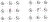
\includegraphics[width=0.5\linewidth]{figures/misc/p_n_type.pdf}
	\caption{Silīcija kristāla 2D izklājums, atomu ārējās čaulas elektroni ir apzīmēti ar punktiem. Pievienojot bora atomu, iegūst p-tipa pusvadītāju (pa kreisi), bet fosfora atomu --- n-tipa pusvadītāju (pa labi).}
	\label{fig:p-n-type}
\end{figure}

Fotoelementa darbība balstās uz iekšējo fotoelektrisko efektu -- parādību, kad elektrons tiek ierosināts ar gaismas kvantu un pāriet no valences zonas uz vadītspējas zonu. Kad tas notiek augšējā slānī (p-tipa pusvadītājā), elektrons atgrūžas no robežas starp slāņiem, kura ir negatīvi lādēta rekombinācijas dēļ. Negatīvi lādētā (no p-tipa pusvadītāja puses) robeža rada potenciālu starpību, kas veicina elektronu kustību pa vadiem uz patērētāju, tādā veidā radot elektrisko strāvu.
\section{Izmantošana pasaulē}

Silīcija Saules paneļu attīstības intensīvākais posms bija apmēram no 1980. līdz 2000. gadam, kad to maksimālā efektivitāte palielinājās no 15\% līdz 25\%
\cite{Sivaram}. Nākamajos 20 gados efektivitātes pieaugums bija gandrīz desmit reizes mazāks. Tiek pētīti arī citi Saules paneļu pusvadītāju veidi, piemēram, kadmija telurīda (\textit{cadmium telluride}, CdTe) vai gallija arsenīda (\textit{Gallium arsenide}, GaAs), tomēr monokristāliskā un polikristāliskā Si Saules paneļi joprojām aizņem lielāko daļu no tirgus, piemēram, Vācijā Si sastādīja vairāk nekā 90\% no Saules paneļu tirgus pēdējo septiņu gadu laikā ~\cite{prognoze}. Tas tādēļ, ka Si ir pieejamāks un lētāks nekā GaAs\cite{hayes_clemens_2015}, un vairāk izpētīts nekā CdTe pusvadītāji~\cite{Sivaram}.

Svarīgi ievērot, ka saules paneļu efektivitāte ir atkarīga no vairākiem faktoriem, kas mainās līdz ar ģeogrāfisko novietojumu: ģeogrāfiskā platuma, gadalaika, mākoņainības un gaisa piesārņojuma. Tātad, detalizēta saules paneļu efektivitātes analīze var būt noderīga katrā valstī, lai precīzāk izvērtētu solārās enerģijas lietošanas perspektīvas tajā. Var minēt dažus šādu pētījumu piemērus.
\begin{itemize}
  \item Indijas pilsētā Bangalorē izpētīja, ka efektivitāte musona un pēc-musona periodos ir augstāka, nekā ziemā un vasarā. To var saistīt ar lielu nokrišņu daudzumu musona periodā, kas labi dzesē Saules paneļus, un ar lielāku saulaino dienu skaitu pēc-musona periodā~\cite{effectCloudsOnSurface}.
  \item Eksperiments Mumbajā ļauj secināt, ka karsts un sauss klimats ne tikai samazina enerģijas pārvērtības lietderības koeficientu, bet arī izraisa defektus un silīcija bojājumus, kas palielina enerģijas zudumus. Tiek norādīts, ka šādā klimatā tipiskais Saules paneļu dzesēšanas risinājums -- ūdens izsmidzināšana -- nav pielietojams, jo tieši šādā klimatā ūdens trūkums ir svarīga problēma~\cite{improvePerformance}.
  \item Indonēzijā pētnieki novēroja, ka mitruma un vēja ātruma palielināšana samazina Saules paneļu efektivitāti~\cite{improvePerformance}~\cite{Sani_2018}. Atšķirībā no iepriekšējā pētījumā, aplūkotajā temperatūras apgabalā (42 -- 52 \textdegree C) temperatūra pozitīvi korelē ar paneļu efektivitāti, kas, iespējams, saistīts ar GHI palielināšanos. 
  \item Arī Latvijā jau ir uzstādītas saules paneļu sistēmas. Piemēram, Ulbrokā 2017. gadā 20 paneļu sistēma kopā saražoja 4554.06 kWh -- vidēji 227.703 kWh gadā no viena paneļa (skat.~\ref{fig:ulbroka}).
\end{itemize}


\begin{figure}[h]
  \centering
  \includegraphics[width=\linewidth]{figures/misc/ulbroka1.pdf}
  \caption{Viena saules paneļa saražotā enerģija Ulbrokas saules paneļu spēkstacijā 2017. gadā. Virziens: D, leņķis 15 \textdegree ~\cite{fronius} (datu nolasīšana: Valts Krūmiņš).}
  \label{fig:ulbroka}
\end{figure}

% otrā nodaļa - saules paneļu uzstādījums LU BD - shēma, utml

\chapter{Saules paneļi LU Botāniskajā dārzā}
% Komentārs: oriģināla metodika, mērījumu/aprēķinu precizitātes novērtējums

\section{Tipi} \label{section:tipi}

% Rindkopa par to, kādi materiāli un ka ir mono un polikristāli un monokristāli labāki un kāpēc.

Botāniskā dārza saules paneļu sistēmu raksturo divi saules paneļu tipi -- JA un LG. Šajā nodaļā saules paneļu tipi tiek salīdzināti savā starpā, gan apskatīti kontekstā ar maksimālo teorētisko efektivitāti.

Ideāli efektīva saules šūna uzņem un iesloga visu krītošo gaismu un 
konvertē to elektriskajos nesējos, kas tiek efektīvi savākti, reālās saules šūnas ir nepilnīgas vienā vai abos no šiem aspektiem. Fundamentālās saules šūnu efektivitātes robeža pēc Šokleja-Ķoizera (\textit{Shockley-Queisser}, S-Q) detalizētā balansa modeļa ir 33.7\%, balstoties uz modeli monokristālisks Si ir sasniedzis $>75\%$ no S-Q robežas, bet polikristālisks Si $50$ līdz $75\%$ no S-Q robežas~\cite{polman2016}.

Monokristāla Si šūnu efektivitātes rekords ir 25.6\%, tās ir sasniegušas gandrīz pilnīgu gaismas slazdošanu un nesēju savākšanu, un lielākoties tās ierobežo nesēja rekombinācijas zudumi. Polikristālisko Si šūnu efektivitātes rekords ir 21.3\%.
% moduļa eff 18.5\%
Polikristālisks Si pusvadītāja plāksnes tiek izgrieztas no stieņa ar virzītās kristalizācijas metodi, un to izgatavošanas izmaksas ir mazākas nekā monokristāliskām plāksnēm. Taču polikristāliskam Si ir zemāka elektroniskā kvalitāte kristāla graudu robežu un iekšgraudu defektu dēļ, kā arī lielāka piemaisījumu koncentrācija, tāpēc polikristāliskai saules šūnai ir lieli sprieguma zudumi. Gaismas slazdošana šajās šūnās ir mazāk efektīva, jo ideālā piramīdas virsmas tekstūra, ko parasti izveido sārmainā kodināšana Si(100) uz (111) virsmas plaknēm, nevar realizēties polikristāliskā virsmā~\cite{polman2016}.
% alkaline-etching Si(100) to (111) surface facets cannot be realized on a multicrystalline surface
% Kontakta rekombinācija reprezentē lielāko daļu zudumu, tāpēc veiksmīgākie risinājumi minimizē saskarsmes laukumu (piem., lokalizēta heavy doping or metal seposition), implementē pasivētus kontkatus vai izmanto šo paņēmienu kombināciju.

Ražotāju referenču lapās LG tiek prognozēta labāka atdeve saulainās dienās~\cite{LGtips}, bet JA labāka atdeve vājas gaismas intensitātes apstākļos~\cite{JAtips}. Ņemot vērā nespēju šos apgalvojumu patiesumu praktiski pārbaudīt patentēto (\textit{proprietary}) modeļu dēļ, atsevišķi izvērtējot tikai \ref{section:clouds}. nod. aprakstītos mākoņainības apsvērumus, Latvijas klimatam piemērotāks būtu JA.

\begin{table}[h]
    \caption{JA un LG paneļu tipu salīdzinājums~\cite{JAtips}~\cite{LGtips}} % uzrakstīt kādu absolūto TSI izmērīja vai norādīt uz grafiku?
    \begin{center}
    \begin{tabular}{| r | c | c |}
    \hline
    Tipa abreviatūra & JA & LG \\ \hline
    Modelis &  JAP60-275/4BB & LG365Q1C-A5\\ \hline
    % materiāls & silikons &   \\ \hline
	Kristāla veids & Polikristālisks & Monokristālisks \\ \hline
	% šūnas izmērs, mm  &156x156  & \\ \hline
	Šūnu skaits  &60  &60 \\ \hline
	Virsmas laukums, $m^2$ &1.64  &1.72 \\ \hline
	STC Pmax, $W$ 	&270 &365\\ \hline
	NOCT Pmax, $W$  &196 &275\\ \hline
	Efektivitāte, \% &16 & 20\\ \hline
    \end{tabular}
    \end{center}
    \label{tab:ja_lg_tipi}
\end{table}

Paneļu maksimālā jauda ($P_{max}$) tiek testēta pie:
\begin{itemize}
\item standarta testa nosacījumiem (\textit{Standart test condition} - STC):\\
Saules izstarojums 1000 W/m$^2$; apkārtējā temperatūra 25\textdegree C.
\item nominālās šūnas darba temperatūras (\textit{Nominal operating cell temperature} - NOCT):\\
Saules izstarojums 800 W/m$^2$; apkārtējā temperatūra 20 \textdegree C; vēja ātrums 1 m/s
\end{itemize}

% ielikt bildi ar to kas saules apstarojumā pazūd no imene

\section{Elektriskā shēma}

Šajā nodaļā tiek paskaidrotas elektroniskās shēmas (skat.\ref{fig:shema}.att.) komponentes un to funkcionalitāte.

\begin{enumerate}
\item Saules baterijas (skat. ~\ref{section:mechanism}. un ~\ref{section:tipi}. nodaļas)
\item \emph{SmartSolar MPPT} --
Saules enerģijas lādētājs savāc enerģiju no saules bateriju paneļiem un noglabā to akumulatoros. Tā mērķis ir novērst bateriju izlādēšanās izraisītos bojājumus. Pirmais skaitlis modeļa nosaukumā apzīmē maksimālo PV slēguma spriegumu, otrais -- maksimālo uzlādes strāvu.
\item Līdzstrāvas drošinātāju skapis -- nepieciešamības gadījumā izolē slēgumu no barošanas avota.
\item \emph{Cyrix-Li-Charge 12/24V -120 A} --
Lādēšanas ierobežotājs atslēdzas, kad tā kontroles izvade kļūs brīvi peldoša (\textit{free floathing}), signalizējot par baterijas pārspriegumu vai paaugstinātu temperatūru. Tas pievieno akumulatora lādētāju ar 3 sekunžu aizkavi, ja VE.Bus BMS lādiņa atvienošanas (\textit{Charge Disconnect}) izvade ir augsta (\textit{high}), spriegums uz akumulatora lādētāja savienojuma spailes ir $\geq 13.7$ V vai spriegums uz akumulatora spailes ir $\geq 2$V.
\item Kūstošais drošinātais --
izkūst pārslodzes gadījumā, novēršot dārgāku instrumentu bojāšanu.
\item \emph{LiFeO4 akumulators 13.8V/90Ah - BMS}
\item Šunts -- mazas pretestības ceļš, ko pieslēdz paralēli galvenajam elektriskās ķēdes posmam, lai tajā samazinātu strāvu. PV sistēmās lietots, lai apietu nevēlamu īssavienojumu starp saules baterijas priekšējo un aizmugurējo virsmas kontaktu, ko parasti izraisa pusvadītāja plāksnes bojājumi.
\item \emph{BMV-702 Smart} --
Akumulatora monitors aprēķina akumulatora spriegumu, strāvas stiprumu, patērēto ampērstundu skaitu, uzlādes stāvokli un atlikušo sistēmas darbības laiku pie pašreizējās izlādes ātruma.
\item \emph{VE.BUS BMS} --
Bateriju vadības bloks pasargā no akumulatoru bojājumiem uzlādes nelīdzsvatorības dēļ. Baterija ar nedaudz lielāku iekšējās noplūdes strāvu
%bateriju bankā ar daudzām virknē vai paralēli savienotām baterijām
izraisīs konkrētās baterijas un paralēli savienoto bateriju nepietiekamu uzlādi un virknē savienoto bateriju pārlādi. Taču virknē savienotām baterijām nepieciešams vienāds sākotnējais uzlādes līmenis. Mazas atšķirības uzlādes līmenī tiks novērstas absorbcijas vai izlīdzināšanās ceļā, bet lielas atšķirības izraisīs bojājumus pārmērīgas pārlādes izraisītas gazifikācijas dēļ baterijām ar lielāku sākotnējo uzlādes līmeni un nepietiekamas uzlādes izraisītās sulfācijas dēļ baterijām ar mazāku sākotnējo uzlādes līmeni.

Bateriju vadības bloks pielīdzina uzlādes līmeni divām bateriju virknēm vai daudzām paralēli savienotām bateriju virknēm. Kad uzlādes spriegums bateriju sistēmai palielinās līdz sistēmā iestatītajai robežai, baterijas vadības bloks salīdzina spriegumus divās virknēs savienotajās baterijās un samazina strāvas padevi akumulatoram (vai paralēli savienotām baterijām) ar augstāko spriegumu. Rezultātā izveidotais uzlādes strāvas diferenciālis nodrošinās, ka visas baterijas konverģēs vienā uzlādes stāvoklī.
% http://www.ultraflexgroup.com/en/catalogue/batteries/09909d-1/1170/vebus-bms.html
% sulfācija - Organiskā savienojuma ūdeņraža atoma aizstāšana ar sulfāta (- OSO2OH) funkcionālo grupu vai divu molekulu ūdeņraža atomu aizstāšana, lai veidotu sulfātu (R-OSO2O-R)
\item \emph{Octo GX} -- instalācijas sakaru centrs ar tālvadības konsoli tiešraides datu uzraudzībai un iestatījumu maiņai, kurai var piekļūt caur Victorn Attālinātās Pārvaldības Portālu(\textit{Victron Remote Management Portal}, VRM) vai lokālo LAN/WiFI tīklu.
% The Octo GX is particularly suited to medium size installations which have many MPPT Solar Chargers, as it has 10 VE.Direct ports
\item \emph{MultiPlus 24/3000/70-16 230V VE.Bus}  --
Autonoms lādētājs pārņēm strāvas padevi tīkla avārijas vai ģeneratora strāva atvienošanās gadījumā $<20$ ms laikā, lai elektroniskās iekārtas turpina darboties bez traucējumiem~\cite{victron}. 
\end{enumerate}

\begin{figure}[h]
    \centering
    \includegraphics[width=0.7\linewidth]{figures/misc/shema.pdf}
    \caption{Saules paneļu elektriskā shēma (autors Valdis Gailītis, modifikācijas Viktorija Leimane)}
    \label{fig:shema}
\end{figure}

\section{Telpiskās orientācijas}

Pēc telpiskās orientācijas saules paneļi tiek iedalīti divās grupās:
\begin{itemize}
\item 13 grādu leņķī (R13, A13, D13)
\item D virzienā (D13, D40, D90)
\end{itemize}

LU Botāniskā dārzā uzstādīto saules paneļu telpiskās orientācijas uzskatāmi parādītas \ref{fig:paneli}. att. (shematiski) un \ref{fig:paneli2}. att. (dabā). Lai lasītājam atvieglotu rezultātu interpretāciju, šīs grupas grafikos tiek apzinātas ar krāsām: leņķu grupa tiek apzīmēta ar zaļo krāsu, D virziena grupa ar zilo, abām grupām kopīgais panelis D13 -- ar tirkīzzilu, krāsu paletes leģenda pieejama \ref{fig:paneli}. att.


\begin{figure}[h]
    \centering
    \includegraphics[width=0.7\linewidth]{figures/misc/krasas_izvietojums.pdf}
    \caption{Saules paneļu telpisko orientāciju shēma (autors Valdis Gailītis, modifikācijas Viktorija Leimane)}
    \label{fig:paneli}
\end{figure}

\begin{figure}[h]
    \centering
    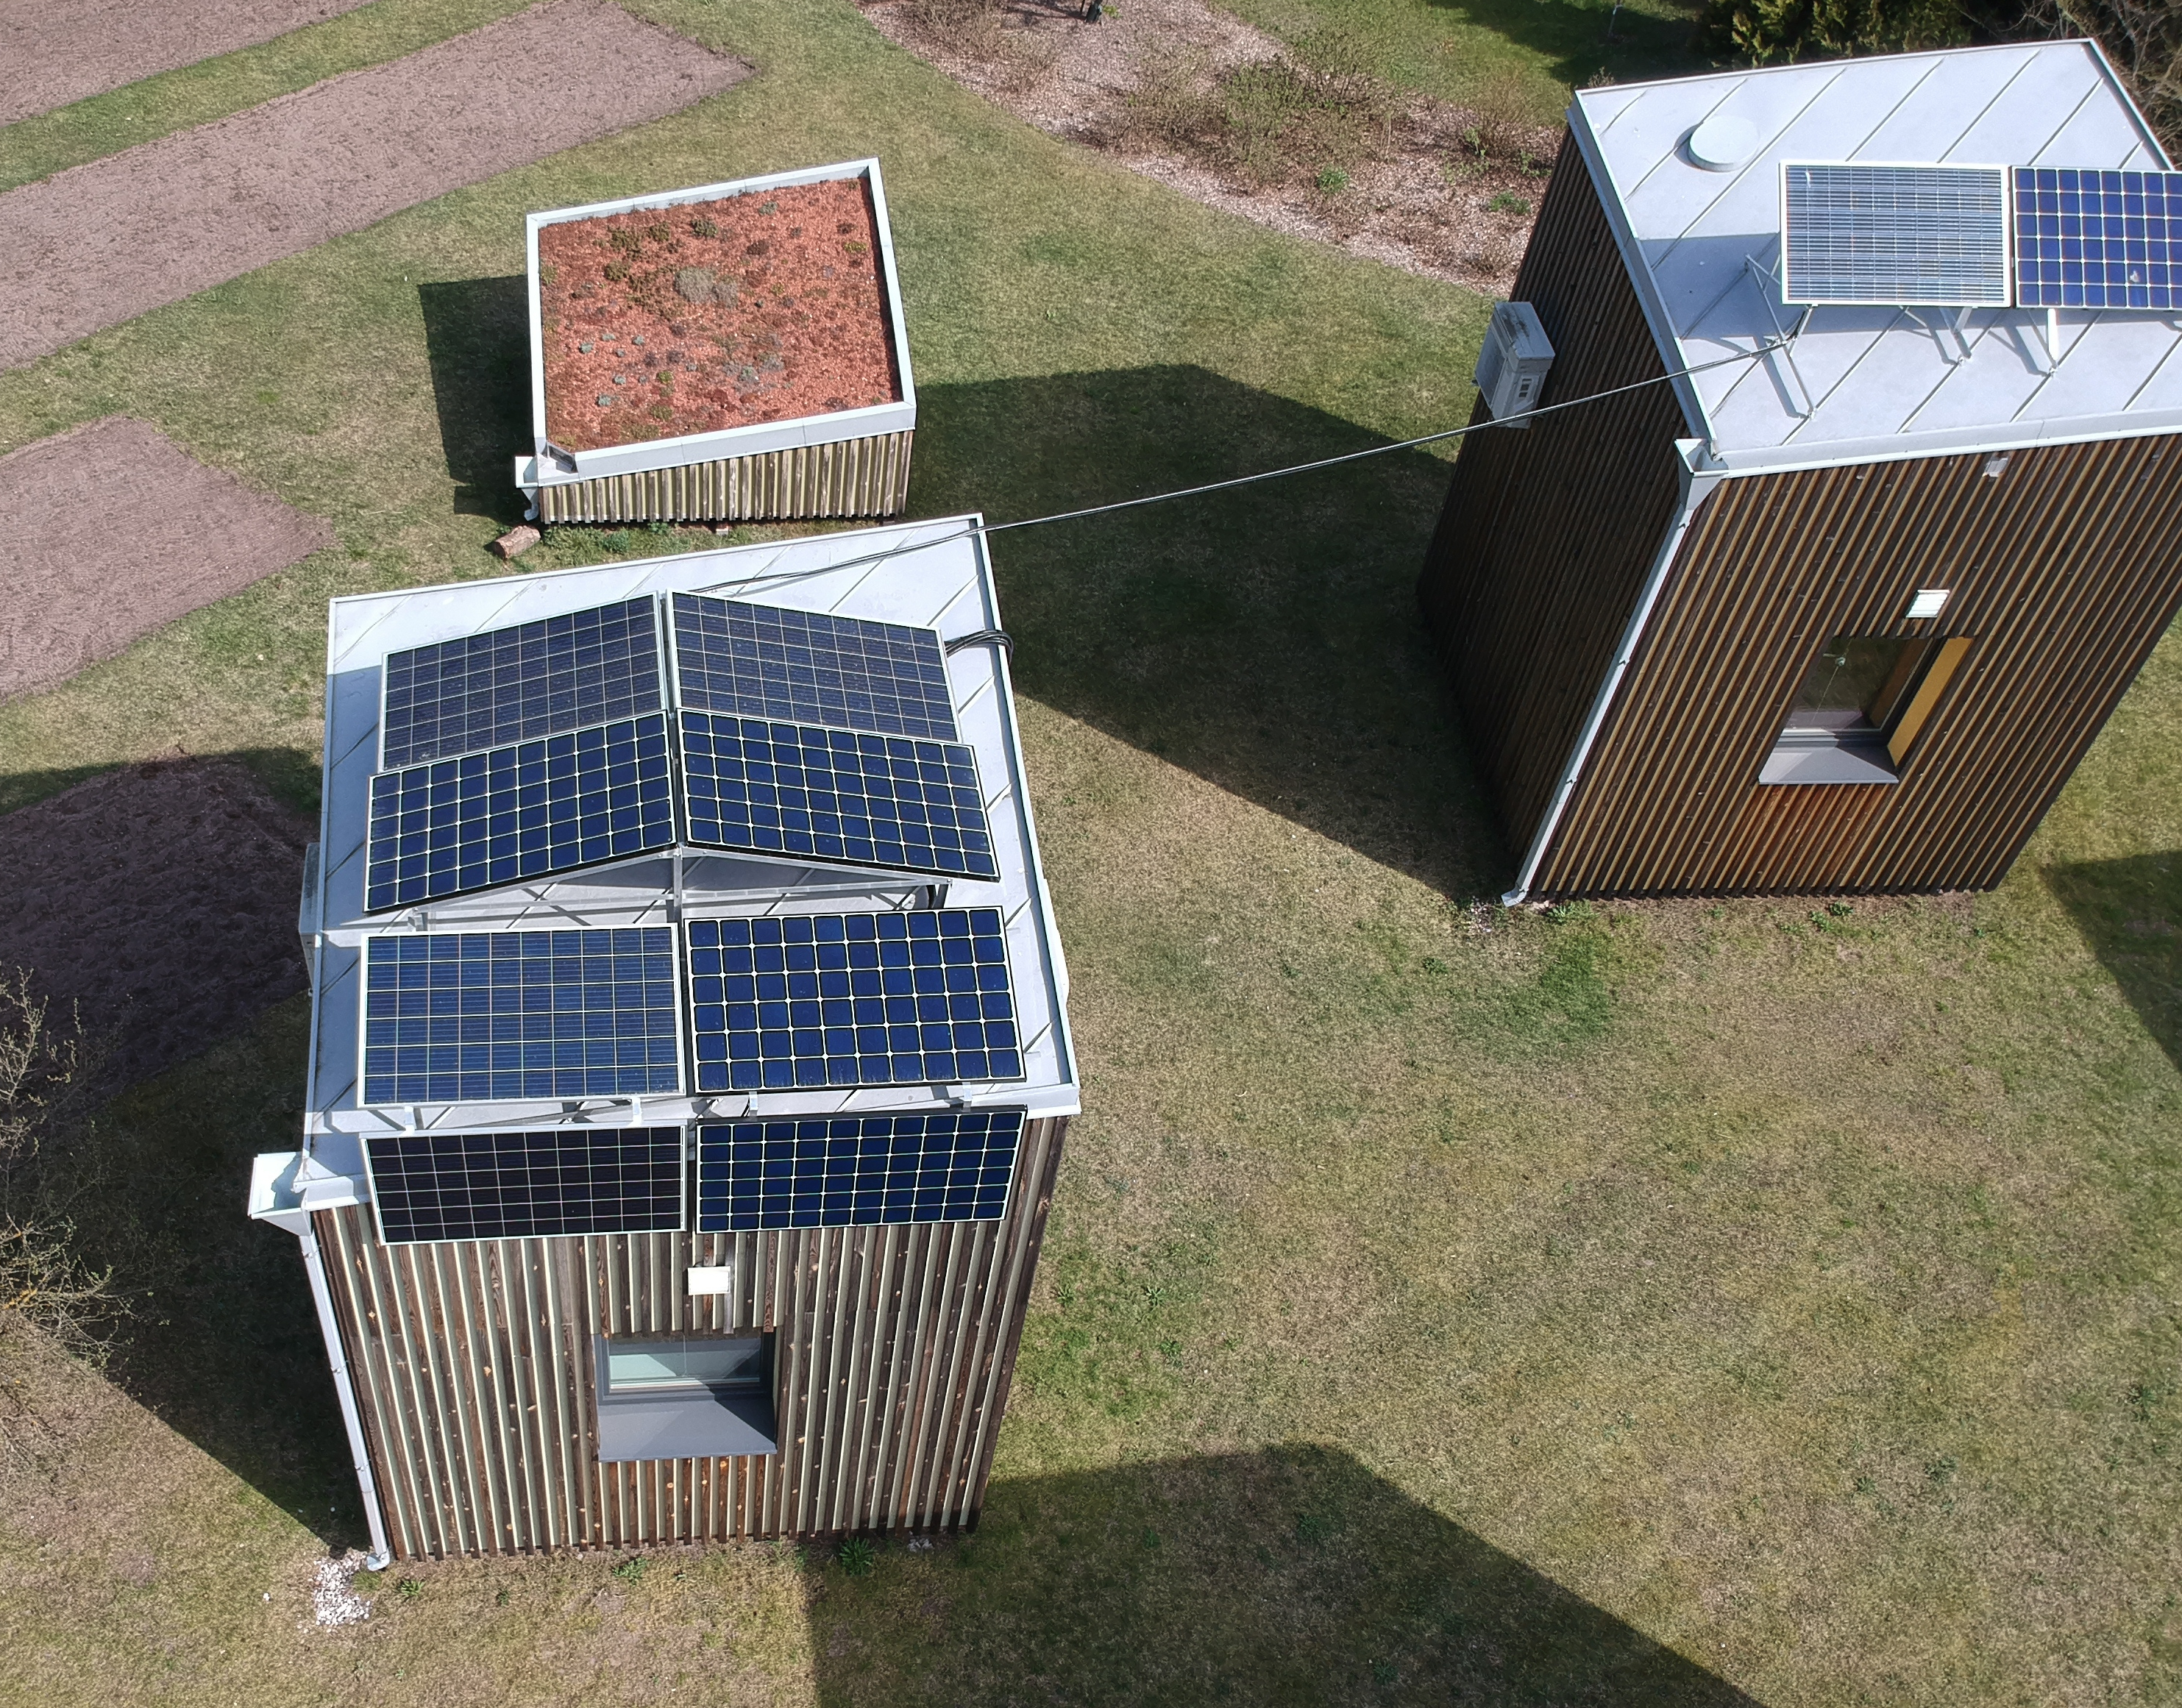
\includegraphics[width=0.7\linewidth]{figures/stenduBildes/overview2.JPG}
    \caption{Saules paneļu telpiskās orientācijas dabā (fotogrāfijas autors Māris Šinka)}
    \label{fig:paneli2}
\end{figure}
\input{tex/kods}

%* Rezultāti
\chapter{Rezultāti}
\input{tex/rezultati}
\section{Saules apstarojums}
% \begin{figure}[h]
%     \centering
%     \includegraphics[width=\linewidth]{figures/meteo/statsYears.pdf}
%     \caption{Solārā apstarojuma laika integrāļa atšķirības gada gaitā. Eksperimentālā poligona meteostacijas stacijas dati 2013 -- 2019 periodā.}
%     \label{fig:metYears}
% \end{figure}

% izlabo visur lu meteoroloģiju uz poligonu
% pārsaukt grafikā Em^-2 uz E_{norm} (normētais enerģijas blīvums)

Tieši ilgtermiņa saules apstarojuma monitorings saules paneļu uzstādīšanas vietā ir svarīgs paneļu efektivitātes prognozēšanas rīks, jo ļauj samazināt anomālu saulaina laika periodu svaru, kādi, piemēram, ir 2014. un 2019. gada aprīļi (skat. \ref{fig:metYears_mean}. att.). PV sistēmas veiktspējas monitoringam lietots Saules apstarojuma sensors (piranometrs), kas atrodas eksperimentālā poligona teritorijā. Šī mērierīce saules apstarojumu uztver ar plaknes virsmu no 180\textdegree skata leņķa, ko sauc par puslodes saules apstarojumu, un tās kļūda ir  $\pm 1 \%$ ~\cite{pyranometer}.

Attēlos \ref{fig:met_Irrad} un \ref{fig:met_Irrad_mean} redzams gaišo diennakts stundu momentānā saules apstarojuma integrāļi 5 minūšu intervālos novēroto četru mēnešu laikā, kas izskaidro turpmāk minētās atšķirības paneļu ražīgumā atkarībā no mēneša -- palielinās gan Saules spīdēšanas ilgums dienā (x ass), gan saņemtās enerģijas daudzums (y ass).

\begin{figure}[h]
    \centering
    \includegraphics[width=\linewidth]{figures/meteo/meanYears.pdf}
    \caption{Solārā apstarojuma laika integrāļa atšķirības gada gaitā un to vidējās vērtības. Eksperimentālā poligona meteostacijas stacijas dati 2013 -- 2019 periodā.}
    \label{fig:metYears_mean}
\end{figure}
\begin{figure}[h]
    \centering
    \includegraphics[width=\linewidth]{figures/meteo/sun19.pdf}
    \caption{Solārā apstarojuma izmaiņas dienas gaitā. Eksperimentālā poligona meteostacijas stacijas dati 2019-01-01 -- 2019-04-31 periodā.}
    \label{fig:met_Irrad}
\end{figure}
\begin{figure}[h]
    \centering
    \includegraphics[width=\linewidth]{figures/meteo/mean19.pdf}
    \caption{Mēnesī vidējotas solārā apstarojuma izmaiņas dienas gaitā. Eksperimentālā poligona meteostacijas stacijas dati 2019-01-01 -- 2019-04-31 periodā.}
    \label{fig:met_Irrad_mean}
\end{figure}
\section{Efektivitātes atkarība no parametriem}
\subsection{Saules paneļa tipa} \label{subsection:tipi}

Pēc tabulām \ref{tab:JA} un \ref{tab:LG}, kā arī grafikiem, kas ietverti diskusijā par citu parametru ietekmi uz efektivitāti (skat. \ref{subsection:gads}. nod.), redzams, ka LG tipa paneļi konsekventi ir efektīvāki par JA tipu. Tas ir saistīts gan ar kristāla veidu -- kā parādīts \ref{section:tipi}. nod.,  monokristāliska Si paneļi ir ražīgāki par polikristāliem --, gan paneļu maksimālajām jaudām -- LG
ir lielāka nominālā jauda uz laukuma vienību nekā JA.

\begin{table}[!htbp]
    \caption{JA tipa paneļu saražotā enerģija uz kvadrātmetru salīdzināta ar\\ enerģijas plūsmas blūvumu uz horizontālu virsmu}
    \begin{center}
    %%%%%%%%%%%%%%%%%%%%%%%%%%%%%%%%%%%%%%%%%%%%%%%%%%%%%%%%%%%%%%%%%%%%%%
%%                                                                  %%
%%  This is a LaTeX2e table fragment exported from Gnumeric.        %%
%%                                                                  %%
%%%%%%%%%%%%%%%%%%%%%%%%%%%%%%%%%%%%%%%%%%%%%%%%%%%%%%%%%%%%%%%%%%%%%%
\begin{tabular}{ | c | r r r r r  r | } \hline
E, $\textrm{kWhm}^{-2}$	&A.13	&R.13	&D.13	&D.40	&D.90	&piranometrs\\ \hline
jan		&0.35	&0.23	&0.72	&2.46	&2.80		&12.14\\
feb		&3.20	&2.74	&4.27	&6.45	&5.99		&25.14\\
mar		&8.22	&7.40	&9.47	&11.94	&8.72		&61.76\\
apr		&19.89	&19.23	&23.27	&25.43	&18.25		&141.41\\ \hline
$E_{sum}$, $\textrm{kWhm}^{-2}$
		&31.7	&29.6	&37.7	&46.3	&35.8 	&240.5\\ \hline
\end{tabular}
    \end{center} \label{tab:JA}
\end{table}
\begin{table}[!htbp]
    \caption{LG tipa paneļu saražotā enerģija uz kvadrātmetru salīdzināta ar\\ enerģijas plūsmas blūvumu uz horizontālu virsmu}
    \begin{center}
    %%%%%%%%%%%%%%%%%%%%%%%%%%%%%%%%%%%%%%%%%%%%%%%%%%%%%%%%%%%%%%%%%%%%%%
%%                                                                  %%
%%  This is a LaTeX2e table fragment exported from Gnumeric.        %%
%%                                                                  %%
%%%%%%%%%%%%%%%%%%%%%%%%%%%%%%%%%%%%%%%%%%%%%%%%%%%%%%%%%%%%%%%%%%%%%%
\begin{tabular}{ | c | r r r r r  r | } \hline
E, $\textrm{kWhm}^{-2}$	&A.13	&R.13	&D.13	&D.40	&D.90 	&piranometrs\\ \hline
jan	&0.5	&0.35	&0.95	&2.82	&3.22		&12.14	\\
feb	&4.43	&3.63	&5.05	&8.25	&7.41		&25.14	\\
mar	&10.92	&9.27	&11.27	&15.69	&11.34		&61.76	\\
apr	&27.63	&25.46	&29.14	&34.21	&23.18		&141.41	\\ \hline
$E_{sum}$, $\textrm{kWhm}^{-2}$
	&43.48	&38.7	&46.41	&60.98	&45.14		&240.46	\\ \hline
\end{tabular}
    \end{center} \label{tab:LG}
\end{table}

% %%%%%%%%%
\subsection{Saules paneļa leņķa}\label{subsection:degree}
Apkopojot četru mēnešu datus un abus paneļu tipus, visražīgākais leņķis ir 40\textdegree ~(skat.~\ref{fig:lg_ja_deg}. att.).
Kopumā var secināt, ka pret D orientētais panelis 90\textdegree ~leņķī saražo vairāk enerģijas ziemas mēnešos un 13\textdegree ~leņķī -- vasaras mēnešos, tātad apstiprinās teorijā (\ref{section:kustiba}.nod.) prognozētais.
% Tas sakrīt ar [ielikt grafiku ar LV karti un optimālo leņķi bet es neatceros no kurienes paņēmu to].
\begin{figure}[h!]
    \centering
    \includegraphics[width=\linewidth]{figures/results/all_degType.pdf}
    \caption{D virzienā vērsto saules paneļu saražotā enerģija atkarībā no leņķa un saules paneļu tipa} \label{fig:lg_ja_deg}
\end{figure}


\subsection{Saules paneļa virziena}\label{subsection:dir}
Visražīgākais virziens ir D, tad A, tad R (skat.~\ref{fig:lg_ja_dir}. att.). To paskaidro \ref{subsection:month_day}. nod. redzamie paneļu saražotās enerģijas dienas sadalījumi.
\begin{figure}[h!]
    \centering
    \includegraphics[width=\linewidth]{figures/results/all_dirType.pdf}
    \caption{13 grādu leņķī vērsto saules paneļu atkarība no virziena un saules paneļu tipa}
    \label{fig:lg_ja_dir}
\end{figure}

\subsection{Saules paneļa leņķa un virziena kombinācijas}
\label{subsection:month_day}

Saules paneļu saņemtā apstarojuma dienas sadalījuma tendenci drīkst salīdzināt ar attiecīgo paneļu saražotās enerģijas tendenci, jo pēdējā ir atkarīga no paneļa virsmas saņemtā Saules apstarojuma, kas savukārt ir funkcija no $cos(\theta)$, tātad proporcionāla tam. Salīdzinot \ref{fig:cos-theta}.(c) ar 
\ref{fig:toldU}, tiek secināts, ka eksperimentālie rezultāti sakrīt ar teoriju.

\begin{figure}[h]
    \centering
    \includegraphics[width=\linewidth]{figures/sol_day/apr_LG_13.pdf}
    \includegraphics[width=\linewidth]{figures/sol_day/apr_LG_D.pdf}
    \caption{Saules paneļu saražotās enerģijas dienas sadalījuma līkne vidējotiem 27-30. aprīļa datiem} \label{fig:toldU}
\end{figure}

Turpmāk apskatīts Saules apstarojuma dienas sadalījums mēnešos. Kā redzams \ref{fig:mar_ar}, \ref{fig:apr_ar}. att., eksperimentāli noteiktais saules paneļu saražotās enerģijas dienas sadalījums sakrīt ar teorētiski prognozēto \ref{fig:cos-theta}. att. kā arī labi novērojamas tā diennakts svārstības 30 dienu laikā.
% \begin{figure}[h]
%     \centering
%     \includegraphics[width=\linewidth]{figures/sol_day/feb_A13JA.pdf}
%     \includegraphics[width=\linewidth]{figures/sol_day/feb_R13JA.pdf}
%     \caption{A un R virzienu saules paneļu 5 minūtēs vidējotu Wh dienas sadalījumi februārī}
%     \label{fig:feb_ar}
% \end{figure}

\begin{figure}[h]
    \centering
    \includegraphics[width=\linewidth]{figures/sol_day/mar_A13JA.pdf}
    \includegraphics[width=\linewidth]{figures/sol_day/mar_R13JA.pdf}
    \caption{A un R virzienu saules paneļu 5 min intervālos integrētu jaudu dienas sadalījumi martā}
    \label{fig:mar_ar}
\end{figure}

\begin{figure}[h]
    \centering
    \includegraphics[width=\linewidth]{figures/sol_day/apr_A13JA.pdf}
    \includegraphics[width=\linewidth]{figures/sol_day/apr_R13JA.pdf}
    \caption{A un R virzienu saules paneļu 5 minūtēs vidējotu Wh dienas sadalījumi aprīlī}
    \label{fig:apr_ar}
\end{figure}

% % \begin{figure}[h]
% %     \centering
% %     \includegraphics[width=\linewidth]{figures/sol_month/feb_Dir_d.pdf}
% %     \includegraphics[width=\linewidth]{figures/sol_month/feb_Deg_d.pdf}
% %     \caption{Saules paneļu saražotā enerģija atkarībā no virziena un leņķa februārī}
% %     \label{fig:feb_degDir}
% % \end{figure}

% % \begin{figure}[h]
% %     \centering
% %     \includegraphics[width=\linewidth]{figures/sol_month/mar_Dir_d.pdf}
% %     \includegraphics[width=\linewidth]{figures/sol_month/mar_Deg_d.pdf}
% %     \caption{Saules paneļu saražotā enerģija atkarībā no virziena un leņķa martā}
% %     \label{fig:mar_degDir}
% % \end{figure}

% % \begin{figure}[h]
% %     \centering
% %     \includegraphics[width=\linewidth]{figures/sol_month/apr_Dir_d.pdf}
% %     \includegraphics[width=\linewidth]{figures/sol_month/apr_Deg_d.pdf}
% %     \caption{Saules paneļu saražotā enerģija atkarībā no virziena un leņķa aprīlī}
% %     \label{fig:apr_degDir}
% % \end{figure}

\subsection{Gada mēneša} \label{subsection:gads}
Pēc \ref{fig:jan_sum}, \ref{fig:feb_sum}, \ref{fig:mar_sum}, \ref{fig:apr_sum}. att., tiek izdarīti secinājumi par saules paneļu ražīguma atkarību no gada mēneša. Janvārī visefektīvākais panelis ir D.90, kas atbilst janvārim raksturīgajam Saules pārvietojumam -- zemu pie horzionta. \ref{fig:feb_sum}. att. redzams, ka februārī D.40 kļūst ražīgāks nekā D.90, tāpat redzams, ka mazāku leņķu paneļi -- R.13 un A.13 -- proporcionali vairāk Saules apstarojuma ir pārvērtuši enerģijā. Šī tendence novērojama arī turpmākajos mēnešos. Savukārt jau aprīlī visefektīvākā orientācija ir D.40. Visu telpisko orientāciju paneļi ir pakļauti Saules diennakts pārvietojuma izmaiņas izraisītajiem efektiem uz saražotās enerģijas apjomu, kas teorētiski aprēķināti \ref{section:kustiba}. nod.

% Janvārī visefektīvākaie ir paneļi, kas orientēti uz dienvidiem un novietoti vertikāli (D.90), jo Saule pārvietojas zemu gar horizontu. Savukārt jau aprīlī visefektīvākā orientācija ir D.40, un arī citu orientāciju paneļi ir pakļaut līdzīgiem efektiem, kas teorētiski aprēķināti \ref{section:kustiba}. nod.

Arī Ulbrokas saules paneļu spēkstacijas darbības analīze gada griezumā (skat. \ref{fig:ulbroka}. att.) uzrāda ļoti būtisku saules paneļu saražotās enerģijas variabilitāti gada mēnešos. Maksimālais enerģijas daudzums tiek saražots maijā, nedaudz mazāk citos vasaras mēnešos, bet janvārī, februārī, novembrī un decembrī saražotās enerģijas daudzums ir ļoti mazs. Šis apsvērums ir īpaši svarīgs industrializētos pielietojumos, jo ziemas mēnešos jādomā par alternatīvu enerģijas avotu.

\begin{figure}[h]
    \centering
    \includegraphics[width=\linewidth]{figures/sol_month/jan_m_m2.pdf}
    \caption{Saules paneļu saražotā enerģija janvārī}
    \label{fig:jan_sum}
\end{figure}

\begin{figure}[h]
    \centering
    \includegraphics[width=\linewidth]{figures/sol_month/feb_m_m2.pdf}
    \caption{Saules paneļu saražotā enerģija februārī}
    \label{fig:feb_sum}
\end{figure}

\begin{figure}[h]
    \centering
    \includegraphics[width=\linewidth]{figures/sol_month/mar_m_m2.pdf}
    \caption{Saules paneļu saražotā enerģija martā}
    \label{fig:mar_sum}
\end{figure}

\begin{figure}[h]
    \centering
    \includegraphics[width=\linewidth]{figures/sol_month/apr_m_m2.pdf}
    \caption{Saules paneļu saražotā enerģija aprīlī}
    \label{fig:apr_sum}
\end{figure}


\section{Salīdzinošā analīze}\label{section:effectivity}

Eksperimentāli noteiktā paneļu efektivitāte (skat.~\ref{tab:eff_type}. tab.) nav pretrunā ne ar ražotāju tehniskajā dokumentācijā doto, nedz teorētiski iespējamo pēc S-Q modeļa. 
% Izmērītā paneļu efektivitāte atšķiras no ražotāju tehniskajā dokumentācijā dotā.
Atšķirības tiek skaidrotas ar efektivitātes mērīšanas veidu -- standarta testi tiek veikti pie konstanta izstarojuma (1000 W/m$^2$ un 800 W/m$^2$) perpendikulāri saules panelim, tomēr reālā poligona apstākļos novērojama starojuma avota kustība pa debesjumu gan diennakts, gan gada ietvaros.

\begin{table}[h!]
    \caption{Katra paneļa eksperimentāli noteiktās efektivitātes vidējā vērtība 4 mēnešu laikā}
    \begin{center}
    %%%%%%%%%%%%%%%%%%%%%%%%%%%%%%%%%%%%%%%%%%%%%%%%%%%%%%%%%%%%%%%%%%%%%%
%%                                                                  %%
%%  This is a LaTeX2e table fragment exported from Gnumeric.        %%
%%                                                                  %%
%%%%%%%%%%%%%%%%%%%%%%%%%%%%%%%%%%%%%%%%%%%%%%%%%%%%%%%%%%%%%%%%%%%%%%
\begin{tabular}{ | c | c c c c c | }\hline
Panelis	&A.13	&R.13	&D.13	&D.40	&D.90\\ \hline
E$_{JA}$, \%		&0.11	&0.10	&0.14	&0.21	&0.18\\ \hline
E$_{LG}$, \%		&0.15	&0.13	&0.17	&0.26	&0.23\\ \hline
\end{tabular}
    \end{center}
    \label{tab:eff_type}
\end{table}

\begin{figure}[h!]
    \centering
    \includegraphics[width=\linewidth]{figures/results/JAm2_w.pdf}
    \caption{JA tipa paneļu saražotais mēnesī salīdzinājumā ar eksperimentālā poligona meteostacijas saules apstarojuma datiem uz horizontālu virsmu (\textcolor{bostonuniversityred}{sarkanā krāsā})}
    \label{fig:ja}
\end{figure}
\begin{figure}[h!]
    \centering
    \includegraphics[width=\linewidth]{figures/results/LGm2_w.pdf}
    \caption{LG tipa paneļu saražotais mēnesī salīdzinājumā ar eksperimentālā poligona meteostacijas saules apstarojuma datiem uz horizontālu virsmu (\textcolor{bostonuniversityred}{sarkanā krāsā})}
    \label{fig:lg}
\end{figure}

\section{Salīdzinājums ar citas saules paneļu spēkstacijas mērījumu rezultātiem}

Tabulās \ref{tab:ja_ul}. un \ref{tab:lg_ul} salīdzināta Botānisko dārzu saules paneļu saražotā enerģija 2019. gada janvārī -- aprīlī ar 2017. gada Ulbrokas spēkstacijas viena paneļa saražoto enerģiju janvāra -- aprīļa periodā. Jāpiebilst, ka spēkstacijām atšķiras lokācijas, turklāt, spriežot pēc, \ref{fig:metYears_mean}. att., 2019. gadā attiecīgajos mēnešos bija krietni lielāks Saules apstarojums, kas izskaidro Ulbrokas paneļu šķietamo neefektivitāti, taču dod ieskatu sistēmas prognozējamā darbībā.
\begin{table}[h]
    \caption{JA tipa paneļu saražotās enerģijas salīdzinājums ar Ulbrokas spēkstacijā saražoto 2017. gadā}
    \begin{center}
    %%%%%%%%%%%%%%%%%%%%%%%%%%%%%%%%%%%%%%%%%%%%%%%%%%%%%%%%%%%%%%%%%%%%%%
%%                                                                  %%
%%  This is a LaTeX2e table fragment exported from Gnumeric.        %%
%%                                                                  %%
%%%%%%%%%%%%%%%%%%%%%%%%%%%%%%%%%%%%%%%%%%%%%%%%%%%%%%%%%%%%%%%%%%%%%%
\begin{tabular}{ | c | c c c c c c | }\hline
E, kWh	&A.13	&R.13	&D.13	&D.40	&D.90 &Ulbroka\\ \hline
jan	&0.57	&0.37	&1.17	&4.02	&4.58	&0.84\\
feb	&5.23	&4.48	&6.98	&10.54	&9.79	&5.62\\
mar	&13.44	&12.1	&15.49	&19.52	&14.26	&15.59\\
apr	&32.52	&31.44	&38.05	&41.57	&29.84	&25.56\\ \hline
E$_{sum}$, kWh	&51.76	&48.4	&61.68	&75.66	&58.47	&47.61\\ \hline
\end{tabular}
    \end{center} \label{tab:ja_ul}
\end{table}
\begin{table}[h]
    \caption{LG tipa paneļu saražotās enerģijas salīdzinājums ar Ulbrokas spēkstacijā saražoto 2017. gadā}
    \begin{center}
    %%%%%%%%%%%%%%%%%%%%%%%%%%%%%%%%%%%%%%%%%%%%%%%%%%%%%%%%%%%%%%%%%%%%%%
%%                                                                  %%
%%  This is a LaTeX2e table fragment exported from Gnumeric.        %%
%%                                                                  %%
%%%%%%%%%%%%%%%%%%%%%%%%%%%%%%%%%%%%%%%%%%%%%%%%%%%%%%%%%%%%%%%%%%%%%%
\begin{tabular}{ | c | c c c c c c | }\hline
E, kWh	&A.13	&R.13	&D.13	&D.40	&D.90 &Ulbroka\\ \hline
jan	&0.86	&0.60	&1.64	&4.87	&5.55	&0.84\\
feb	&7.65	&6.26	&8.72	&14.26	&12.80	&5.62\\
mar	&18.86	&16.01	&19.47	&27.11	&19.58	&15.59\\
apr	&47.73	&43.97	&50.32	&59.09	&40.03	&25.56\\ \hline
E$_{sum}$, kWh	&75.09	&66.85	&80.15	&105.32	&77.97	&47.61\\ \hline
\end{tabular}
    \end{center}\label{tab:lg_ul}
\end{table}


%* Secinājumi
\chapter*{Secinājumi}
\addcontentsline{toc}{chapter}{Secinājumi}
Darba laikā tika apgūtas ggplot2, tidyr, lubridate un dplyr bibliotēkas, ar kuru palīdzību tika atlasīts, analizēts un apkopots liels datu apjoms par 10 saules paneļu darbību no 2019. gada 1. janvāra līdz 30. aprīlim.

Darbā iegūtie rezultāti ļauj izdarīt secinājumus, ka no sistēmā esošajiem parametriem efektīvākā kombinācija ir:
\begin{itemize}
	\item 40 grādu leņķis
	\item D virziens
	\item LG panelis
	\item aprīļa mēnesis
\end{itemize}

% KĻŪDAS!!!?????????

Saules paneļu efektivitātes dziļāka izpratne pieprasa tālākus pētījumus, it īpaši nolietojuma, putekļu, vēja, nokrišņu un citu apstākļu ietekmes izpētei.

%* Pateicības
\chapter*{Pateicības}
\addcontentsline{toc}{chapter}{Pateicības}
Pateicos paroksetīnam, xanax, GNU/Linux, Pētera Draguna dzejas krājumam 'Tumšās stundas', Tarvi Verro for teaching me git, Valtam Krūmiņam par emocionālo atbalstu, Žeņam par kucēnu video, Solvitai par maģiju un Cilvēkam par pacietību. Paldies "Puratos Latvia" un Asjas un Berndta Everts piemiņas fondam par stipendiju studiju laikā.

Darbs veikts ar Eiropas Reģionālās attīstības fonta projekta "Viedo risinājumu gandrīz nulles enerģijas ēkām izstrāde, optimizācija un ilgtspējas izpēte reāla klimata apstākļos" Nr ESS2017/209 1.1.1.1/16/A/192 finansiālo atbalstu.


%* Izmantotā darba literatūra un avoti
\clearpage
\addcontentsline{toc}{chapter}{Izmantotā literatūra un avoti}
\printbibliography[title=Izmantotā literatūra un avoti]

%%% Pielikumi
% \appendix

\clearpage

\appendix
\chapter*{Pielikums}
\addcontentsline{toc}{chapter}{Pielikums}
% the \\ insures the section title is centered below the phrase: AppendixA
\noindent {\large \textbf{Autora rezultātu dalība konferencēs}}
\begin{itemize}
\item Zinātniski praktisks seminārs "Ceļā uz gandrīz nulles enerģijas ēkām (gNEĒ) Latvijā". \emph{LU eksperimentālā poligona monitoringa jaunumi: energoefektivitāte un solārā enerģija}. Rīga, Latvija, 2019.g. 11. aprīlis (prezentācija).
% autors: Viktorija Leimane; prezentēja: Andris Jakovičs
\item 7th European conference on renewable energy systems. \emph{The role of solar panel arrangement on their efficency in typical for Latvia weather conditions}. 2019. g. 10.--12. jūnijs, Madride (prezentācija).
\end{itemize}

\noindent {\large \textbf{Izveidotās datu apstrāde sistēmas darbības principu paraugs}}
\input{tex/kods}

% Dokumentālā lapa
\makedoklapa

\end{document}
